\documentclass{beamer}

% Some common packages
\usepackage{graphicx, color}
\usepackage{alltt}
\usepackage{booktabs, calc, rotating}
\usepackage[round]{natbib}
\usepackage{multicol}
\usepackage{amsmath, amsbsy, amssymb, amsthm, graphicx}
\usepackage[english]{babel}
\usepackage{xkeyval} 
\usepackage{xfrac}
\usepackage[normalem]{ulem}
\usepackage{fancyvrb} 
\usepackage{tikz, geometry, tkz-graph, xcolor}
\usepackage[latin1]{inputenc}
\usepackage{times}
\usepackage[T1]{fontenc}

% Shortcuts
\newcommand{\empr}[1]{{\emph{\color{red}#1}}}
\newcommand{\cov}{\mathrm{cov}}
\newcommand{\pkg}[1]{{\textbf{\texttt{#1}}}}
\newcommand{\dif}{\mathrm{d}}
\newcommand{\bigbrk}{\vspace*{2in}}
\newcommand{\smallbrk}{\vspace*{.1in}}
\newcommand{\midbrk}{\vspace*{1in}}
\newcommand{\red}[1]{{\color{red}#1}}
\newcommand{\blue}[1]{{\color{blue}#1}}
\newcommand{\green}[1]{{\color{green}#1}}
\newcommand{\calc}[1]{{\fbox{\mbox{#1}}}}
\newcommand{\Var}{\mathrm{Var}}%
\newcommand{\Cov}{\mathrm{Cov}}%

\mode<presentation>
{
	\usetheme{UTD}
	\usecolortheme[RGB={200,0,0}]{structure}
	\setbeamercovered{transparent}
}

% fancy for Verbatim?
\fvset{frame=single,framesep=1mm,fontfamily=courier,fontsize=\scriptsize,numbers=left,framerule=.3mm,numbersep=1mm,commandchars=\\\{\}}


\title[Survival Analysis]{Applied Survival Analysis Using R\\ Chapter 9: Multiple Survival Outcomes and Competing Risks}
\author[Qi Guo]{Qi Guo}
\institute[UTD]{Department of Mathematical Sciences \\ 
	The University of Texas at Dallas}
\date{April, 17 2019}
	
\begin{document}

\begin{frame}
  \titlepage
\end{frame}

% Set up UTD backgroud
\setbeamercolor*{item}{fg=red}
\bgroup
\usebackgroundtemplate{
\tikz[overlay,remember picture] \node[opacity=0.05, at=(current page.center)] {
   
\includegraphics[height=\paperheight,width=\paperwidth]{UTDbg}};}


\section[Outline]{}
\begin{frame}
  \tableofcontents
\end{frame}

\section{Clustered Survival Times}
\begin{frame}
\frametitle{Problem}
\begin{itemize}
\item The type of survival data commonly we have considered has, as \empr{an endpoint}, \empr{a single cause of death}, and the survival times of each case have been assumed to be \empr{independent}.
\item  Problem:
\begin{itemize}
\item How about the independence assumption no longer holds in clustered data?
\item How about the event may repeat indefinitely, and then we would have multiple times per person?
\item How about only the first of several outcomes is observable?
\end{itemize}
\end{itemize}
\end{frame}

\pagebreak
\begin{frame}[fragile]
\frametitle{Example}
\begin{problock}{mutation carrier in female relatives among families}
Determine if a female was a mutation carrier, and find the relationship between mutation and breast cancer, this subset consists of 1,960 families with two or more female relatives; for those with three or more female relatives, two were selected at random. 
\end{problock}
\begin{itemize}
\begin{Verbatim}
> ashkenazi[ashkenazi$famID %in% c(1, 9, 94), ]
   famID    brcancer    age    mutant
1      1           0     73         0 
2      1           0     40         0 
7      9           0     89         0 
8      9           1     60         0 
87    94           1     44         1 
88    94           0     45         1 
\end{Verbatim}
\item And we know the covariate is ``\texttt{mutant}'' ,the censoring variable is ``\texttt{brcancer}''.
\end{itemize}
\end{frame}

\section{Marginal Survival Models}
\begin{frame}
\frametitle{Model}
\begin{itemize}
\item Suppose that there is only one covariate, and its estimate is $\hat{\beta}$,\empr{ignoring} the cluster structure first.
\item Denote the estimate of its variance (from the Cox model) by $\hat{V}$, and the standard error of the estimate is then $\hat{V}^{1/2} = \sqrt{\hat{V}}$. and assume all subjects are independent.
\item To obtain a correction due to the clustering structure, define a 
\empr{score residual} for subject $j$ in cluster $i$:
\begin{equation}
s_{ij} = \delta_{ij}[z_{ij}-\bar{z}(t_{ij})] - \sum\limits_{t_{u}\le t_{ij}}^{}[z_{i}-\bar{z}(t_{ij})]e^{z_i\beta}\big[\hat{H_0}(t_{u}) - \hat{H_0}(t_{u - 1}) \big]
\end{equation}
\end{itemize}
\end{frame}

\pagebreak
\begin{frame}
\frametitle{Model}
\begin{itemize}
\item The first part of this residual is the \empr{Schoenfeld residual} in Chapter 7
\item Formulate a quantity $C$ defined by:
\begin{equation}
C = \sum\limits_{i=1}^{G}\sum\limits_{j=1}^{n_i}\sum\limits_{m=1}^{n_i}s_{ij}s_{im}
\end{equation}
\item We can define a cluster-adjusted variance by $V^{*} = {\hat{V}}^2\cdot C$, and a standard error for $\hat{\beta}$ by $\sqrt{V^{*}}
$.
\item If there are $q$ covariates, $se(\beta) = [diag(V^{*})]^{1/2}$, and the score residuals $s_{ij}$ are $1 \times q$ matrices, $C = \sum\limits_{i=1}^{G}\sum\limits_{j=1}^{n_i}\sum\limits_{m=1}^{n_i}\underset{\sim}{s'_{ij}}\underset{\sim}{s_{im}}$, and the cluster-adjusted covariance matrix is given by $V^{*} = \hat{V}C\hat{V}$.
\end{itemize}
\end{frame}

\section{Frailty Survival Models}
\begin{frame}
\frametitle{Generalize to clustered survival data}
\begin{itemize}
\item The independent survival data, with the $i$th observation given by $(t_i,\delta_i,z_i)$, the likelihood function:
\begin{equation}
L(\beta;z_i) = \prod\limits_{i=1}^{n}f(t_i,\beta)^{\delta_i}S(t_i,\beta)^{1-\delta_i} = \prod\limits_{i=1}^{n}h(t_i,
\beta)^{\delta_i}S(t_i,\beta)
\end{equation}
or in baseline cumulative hazard:
\begin{equation}
L(\beta;z_i) = \prod\limits_{i=1}^{n}[h_0(t_i)e^{z_i\beta}]^{\delta_i}\cdot e^{-H_0(t_i)}e^{z_i\beta}
\end{equation}
where $H_0(t_i) = - \int_{0}^{t_i} h_0(v)dv$ is the baseline cumulative hazard.
\item Now suppose that the survival times are organized into clusters
\end{itemize}
\end{frame}

\pagebreak
\begin{frame}
\frametitle{Generalize to clustered survival data}
\begin{itemize}
\item Assign each individual in a cluster a common factor known as a \empr{frailty} or, alternatively, as a \empr{random effect}, and denote the frailty for all individuals in the $i$th cluster by $\omega_i$, then the hazard function for the $j$th subject in the $i$th cluster as follows:
\begin{equation}
h_{ij}(t_{ij}) = h_0(t_{ij})\cdot \omega_i	e^{z_{ij}\beta}
\end{equation}
and $\omega_i$ is vary from one cluster to another, and a common model that governs this variability is a \empr{gamma distribution}
\begin{equation}
g(\omega_i,\theta) = \frac{\omega^{\frac{1}{\theta}-1}e^{-\frac{\omega}{\theta}}}{\Gamma(\frac{1}{\theta})\theta^{\frac{1}{\theta}}}
\end{equation}
\end{itemize}
\end{frame}


\pagebreak
\begin{frame}
\frametitle{Generalize to clustered survival data}
\begin{itemize}
\item When we take frailties $\omega_i$ into consideration, the the joint likelihood for the $j$th subject in the $i$th cluster would be:
\begin{equation}
L_{ij}(\beta,\theta;\omega_i,t_{ij},\delta_{ij},z_{ij}) = g(\omega_i,\theta)\cdot {[h_0(t_{ij})\omega_i e^{z_{ij}\beta}]}^{\delta_{ij}}\cdot e^{-H_0(t_{ij})\omega_i e^{z_{ij}\beta}}
\end{equation}
and the full likelihood would be:
\begin{equation}
L(\beta,\theta) = \prod\limits_{i=1}^{G}\prod\limits_{j=1}^{n_i}L_{ij}(\beta,\theta;\omega_i,t_{ij},\delta_{ij},z_{ij})
\end{equation}
\item The frailties are \empr{latent} variables, we cannot directly observe. Thus, to obtain estimates of $\beta$ and $\theta$ we need to use a multistage procedure called the \empr{EM (expectation-maximization) algorithm}.
\end{itemize}
\end{frame}

\pagebreak
\begin{frame}[fragile]
\frametitle{Example}
\begin{itemize}
\item Using standard Cox proportional hazards model to predict the age of onset of breast cancer depending on mutant.
\begin{Verbatim}
> result.coxph <- coxph(Surv(age, brcancer) ~ mutant, 
data=ashkenazi)
> summary(result.coxph)
 n= 3920, number of events= 473
           coef    exp(coef)    se(coef)    z       Pr(>|z|) 
mutant    1.1907    3.2895       0.1984    6.002    1.95e-09 ***
\end{Verbatim}
\item The log partial likelihood from this model is obtained as follows:
\begin{Verbatim}
result.coxph$loglik
[1] -3579.707   -3566.745
\end{Verbatim}
\item -3579.707 is no covarites and the -3566.745 is model with ``\texttt{mutant}'' included as a predictor, the likelihood ratio test statistic is twice the difference, $G^2 = 2(3579.707-3566.745)\linebreak=25.924$,compared to a chi-square distribution with 1 df.
\end{itemize}
\end{frame}

\pagebreak
\begin{frame}[fragile]
\frametitle{Model with cluster}
\begin{itemize}
\begin{Verbatim}
> result.coxph.cluster <- coxph(Surv(age, brcancer) ~ mutant +
cluster(famID), data=ashkenazi)
> summary(result.coxph.cluster)
n= 3920, number of events= 473
         coef   exp(coef)  se(coef)  robust.se   z    Pr(>|z|) 
mutant  1.1907   3.2895     0.1984     0.2023  5.886  3.96e-09 ***
\end{Verbatim}
\item The ``\texttt{robust se}'', this estimate is only slightly higher than the one from the standard Cox model, indicating that the effect of clustering within first-degree relatives is small.
\begin{Verbatim}
> result.coxph.frail <- coxph(Surv(age, brcancer) ~ mutant +
frailty(famID), data=ashkenazi)
> summary(result.coxph.frail)
      n= 3920, number of events= 473
               coef  se(coef)    se2    Chisq    DF     p 
mutant        1.272   0.2317   0.2004   30.13   1.0  4.0e-08
frailty(famID)                         221.50 211.6  3.1e-01
\end{Verbatim}
\end{itemize}
\end{frame}

\pagebreak
\begin{frame}[fragile]
\frametitle{New facility in \texttt{R}}
\begin{itemize}
\item The ``\texttt{frailty}'' option, is the ``\texttt{coxme}'' package,must be separately downloaded and installed.
\begin{Verbatim}
> library(coxme)
> result.coxme <- coxme(Surv(age, brcancer) ~ mutant + (1|famID), 
data=ashkenazi)
> summary(result.coxme)    
Cox mixed-effects model fit by maximum likelihood
  Data: ashkenazi events, 
  n = 473, 3920
  Iterations= 10 63           
                    NULL     Integrated     Fitted
Log-likelihood  -3579.707    -3564.622   -3411.522    
                  Chisq    df       p         AIC      BIC
Integrated loglik 30.17   2.0   2.8100e-07   26.17    17.85 
Penalized loglik 336.37  150.1  2.2204e-16   36.16   -588.13
Model:  Surv(age, brcancer) ~ mutant + (1 | famID)
Fixed coefficients
           coef     exp(coef)     se(coef)    z       p 
mutant   1.236609    3.443914    0.2205358   5.61   2.1e-08
Random effects
 Group Variable   Std Dev   Variance 
 famID Intercept 0.5912135  0.3495334      
\end{Verbatim}
\end{itemize}
\end{frame}

\section{Cause-Specific Hazards}
\begin{frame}[fragile]
\frametitle{Kaplan-Meier Estimation with Competing Risks}
\begin{itemize}
\item A patient may potentially experience \empr{multiple events}, only the first-occurring of which can be observed, eg: diagnosis with prostate cancer until death from that Cause 1 to Cause 2, but for a particular patient we can only observe the time to the first event.
\item One way:Select each as the primary event, and to treat the other as a censoring event.
\item However,Obtain unbiased estimates of survival curves, this simplistic method would require the usually \empr{false assumption} that the two causes of death are independent.
\end{itemize}
\end{frame}

\pagebreak
\begin{frame}
\frametitle{Kaplan-Meier Estimation with Competing Risks}
\begin{figure}[h!]
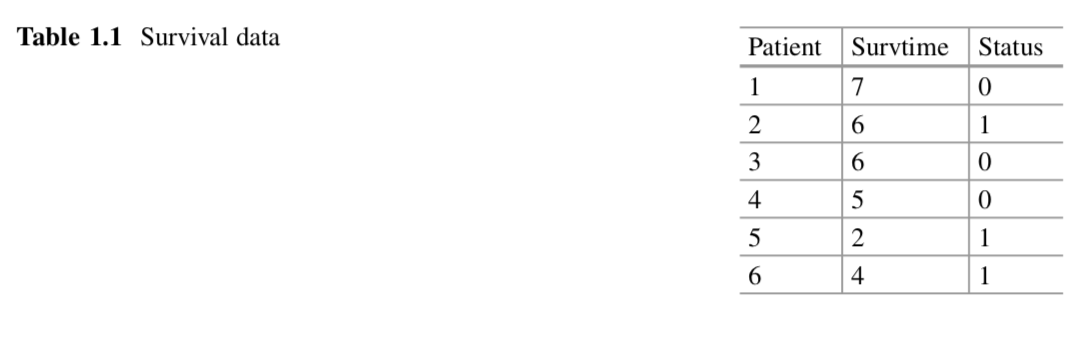
\includegraphics[scale = .5]{001.png}
\end{figure}
\begin{itemize}
\item Skip the R codes, and the result shows above, but such an exercise would require the assumption that the causes be independent. This assumption cannot be tested from the data,
\end{itemize}
\end{frame}

\pagebreak
\begin{frame}
\frametitle{Cause-Specific Hazards and Cumulative Incidence Functions}
\begin{itemize}
\item Suppose that there are K distinct causes of death, and each subject can experience at most one of the K causes of death
\item With competing risks, it is helpful to define, for each cause of interest, a function known as the \empr{cumulative risk function}
\begin{equation}
F_j(t) = Pr(T\le t, C=j) = \int_{0}^{t} h_j(u)S(u) du
\end{equation}
\item And the hazards is:
\begin{equation}
h_j(t) = \lim\limits_{\delta \to 0}\bigg( \frac{Pr(t<T<t+\delta,C=j|T>t)}{\delta}\bigg)
\end{equation}
\item It's easy to get:
\begin{equation}
h(t) = \sum\limits_{j=1}^{K}h_j(t)
\end{equation}
\end{itemize}
\end{frame}

\pagebreak
\begin{frame}
\frametitle{Formula}
\begin{itemize}
\item Suppose now that we have $D$ distinct ordered failure times $t_1$ ,$t_2$,..., $t_D$, estimate the hazard at the $i$th time ti using $\hat{h}(t_i)=d_i/n_i$
\item The cause-specific hazard for the $k$th hazard may be written in a similar form as ${\hat{h}}_k(t_i) = d_{ik}/n_i$
\item The probability of failure from any cause at time $t_i$ is the product of $\hat{S}(t_{i-1})$, the probability of being alive just before $t_i$, and $\hat{h}(t_i)$, the risk of dying at $t_i$. Similarly, the probability of failure due to cause $k$ at that time is $\hat{S}(t_{i-1})\hat{h}(t_i)$
\item So the \empr{cumulative incidence function} is:	
\begin{equation}
{\hat{F}}_k(t) = \sum\limits_{t_i \le t}^{}{\hat{S}(t_{i-1})\hat{h}(t_i)}                                
\end{equation}
\end{itemize}
\end{frame}

\pagebreak
\begin{frame}[fragile]
\frametitle{Example}
\begin{itemize}
\item First compute the overall survival distribution.
\begin{Verbatim}
> tt <- c(2,7,5,3,4,6)
> status <- c(1,2,1,2,0,0)   
> status.any <- as.numeric(status >= 1)
> result.any <- survfit(Surv(tt, status.any) ~ 1)
> result.any$surv
[1] 0.8333333 0.6666667 0.6666667 0.4444444 0.4444444 0.0000000
\end{Verbatim}     
\item Compute the cumulative incidence functions as in the following table:                      
\end{itemize}
\begin{figure}[h!]
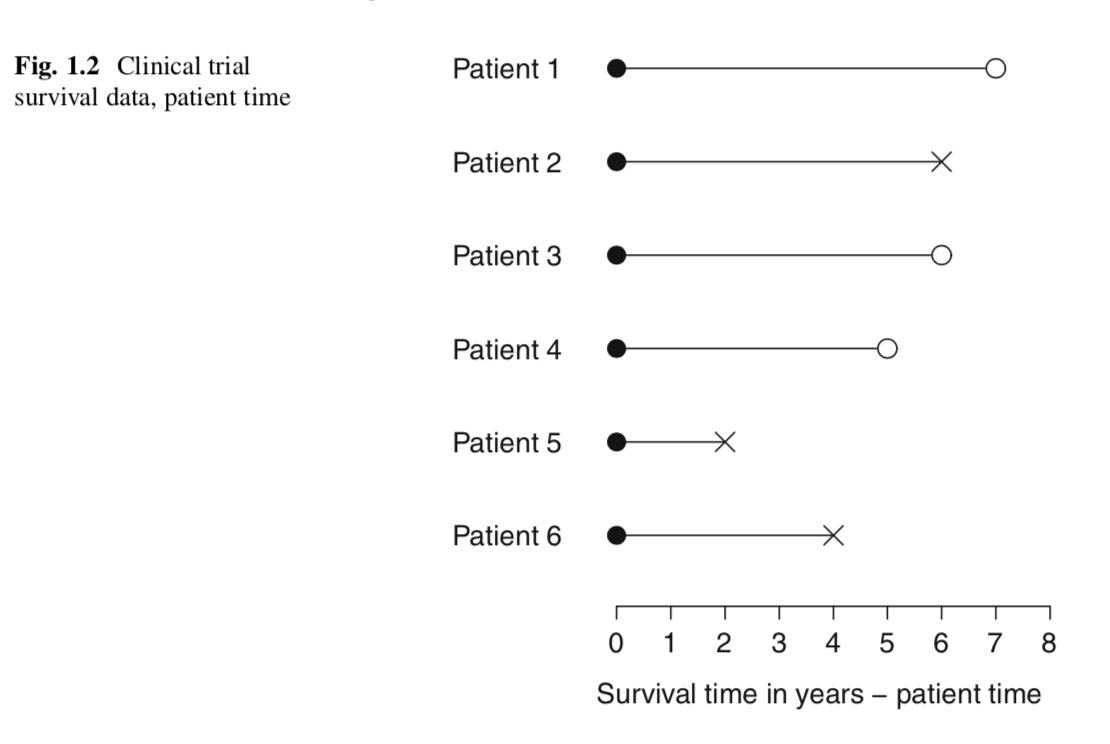
\includegraphics[scale = .4]{002.png}
\end{figure}
\end{frame}



\pagebreak
\begin{frame}[fragile]
\frametitle{Example}
\begin{itemize}
\item Returning to the prostate cancer example of Fig. 9.1,now estimate the competing risks cumulative incidence functions as follows:
\begin{Verbatim}
> sf <- survfit(Surv(survTime, status, type="mstate") ~ 1,
data=prostateSurvival.highrisk)
> tt <- sf$time
> CIs <- sf$pstate 
> ci1 <- CIs[,1] 
> ci2 <- CIs[,2] 
> times <- tt/12 
> Rci2 <- 1 - ci2
\end{Verbatim}     
\item Plot                  
\begin{Verbatim}
> plot(Rci2 ~ times, type="s", ylim=c(0,1),lwd=2, color="green",
xlab="Time in years". ylab="Survival probability")
> lines(ci1~times, type="s", lwd=2, col="blue")
> lines(surv.other.km ~ time.km, type="s",
col="lightgreen", lwd=1)
> lines(cumDist.prost.km ~ time.km, type="s",
col="lightblue", lwd=1)
\end{Verbatim} 
\end{itemize}
\end{frame}


\pagebreak
\begin{frame}
\frametitle{Example}
\begin{figure}[h!]
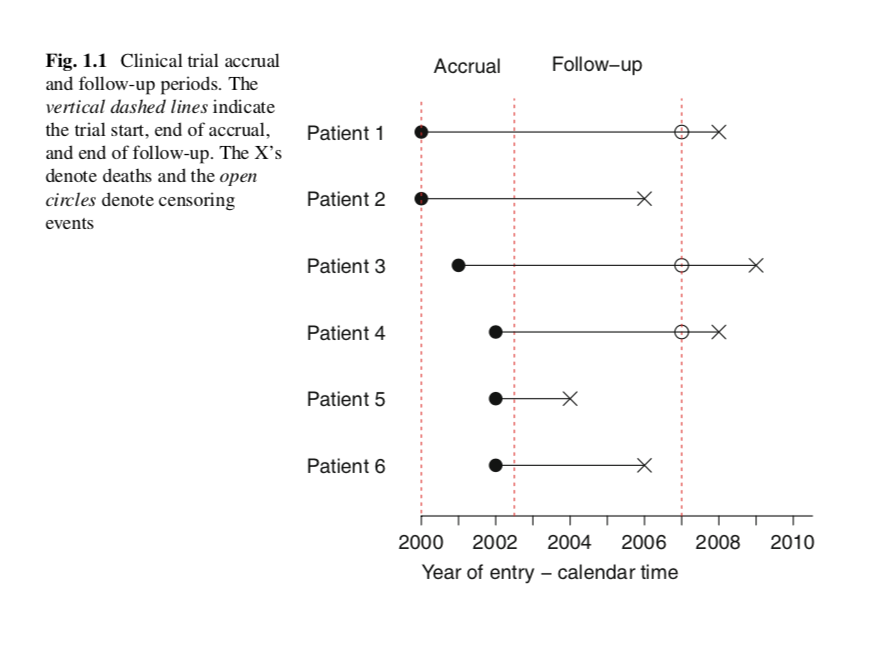
\includegraphics[scale = .5]{003.png}
\end{figure}
\begin{itemize}
\item These curves represent estimates of the actual probabilities that a patient will die of a \empr{particular cause}, rather than hypothetical probabilities that he would die of one cause in the absence of the other.                 
\end{itemize}
\end{frame}

\pagebreak
\begin{frame}[fragile]
\frametitle{Regression Methods for Cause-Specific Hazards}
\begin{itemize}
\item Modeling covariate information for competing risks too difficult to define precisely the hazard function on which the covariates should operate.
\item  Study the effects of the, \empr{remaining covariates (grade and age)} on prostate cancer death, treating other causes of death as censoring indicator.
\begin{Verbatim}
> prostateSurvival.T2 <- prostateSurvival[prostateSurvival$stage 
=="T2",]
> attach(prostateSurvival.T2)  
> result.prostate <- coxph(Surv(survTime, status.prost) ~ grade +
ageGroup)
> summary(result.prostate)
                  coef    exp(coef)   se(coef)    z     Pr(>|z|) 
gradepoor        1.2199    3.3867      0.1004   12.154  < 2e-16 ***
ageGroup70-74   -0.2860    0.7513      0.2595  -1.102   0.2704
ageGroup75-79    0.4027    1.4958      0.2257   1.784   0.0744 
ageGroup80+      0.9728    2.6454      0.2148   4.529   5.92e-06 ***
\end{Verbatim}    
\end{itemize}
\end{frame}


\pagebreak
\begin{frame}
\frametitle{Regression Methods for Cause-Specific Hazards}
\begin{itemize}
\item Conclusion:Patients having poorly differentiated disease (grade = poor) have much worse prognosis than do patients with moderately differentiated disease (the reference group here), with a log-hazard ratio of 1.2199.
\item Define a ``\texttt{sub-distribution hazard}''
\begin{equation}
\bar{h_k}(t) =  \lim\limits_{\delta \to 0} \frac{pr(t<T_k<t+\delta|E)}{\delta}
\end{equation}
where the conditional event is given by:
\begin{equation}
E = \big\lbrace \lbrace T_k >t \rbrace or \lbrace T_{k'} \le t \ and\ k' \neq k \rbrace \big\rbrace
\end{equation}
\end{itemize}
\end{frame}



\pagebreak
\begin{frame}[fragile]
\frametitle{Example}
\begin{itemize}
\item When computing these sub-distribution hazards, the risk set includes not only those currently alive and at risk for the $k$th event type, but also those who \empr{died earlier of other causes}.
\item This method is implemented in the ``\texttt{crr}'' function in the R package ``\texttt{cmprsk}''.
\begin{Verbatim}
> cov.matrix <- model.matrix(~ grade + ageGroup)
> head(cov.matrix)
(Intercept)  gradepoor  ageGroup70-74  ageGroup75-79  ageGroup80+
1      1         0           1               0             0
2      1         1           0               1             0
3      1         1           0               1             0
4      1         1           0               0             1
5      1         0           0               1             0
6      1         0           0               1             0	
> cov.matrix.use <- cov.matrix[,-1] # drop the first column
\end{Verbatim}  
\end{itemize}
\end{frame}


\pagebreak
\begin{frame}[fragile]
\frametitle{Example}
\begin{itemize}
\item Obtain estimates for the prostate cancer as follows, dropping the first (intercept) column of the covariate matrix.
\begin{Verbatim}
> library(cmprsk)
> result.prostate.crr <- crr(survTime, status, cov1=cov.
matrix[,-1], failcode=1)
                  coef   exp(coef)  se(coef)  z     Pr(>|z|) 
gradepoor        1.132    3.102      0.101  11.20   0.00000
ageGroup70-74   -0.272    0.762      0.253  -1.08   0.28000
ageGroup75-79    0.367    1.443      0.219   1.67   0.09400
ageGroup80+      0.799    2.224      0.208   3.85   0.00012
\end{Verbatim}  
\item The argument ``\texttt{failcode=1}'' refers to death from prostate cancer. For death from other causes, we use ``\texttt{failcode=2}'',
\end{itemize}
\end{frame}


\pagebreak
\begin{frame}[fragile]
\frametitle{Comparing the Effects of Covariates on Different Causes of Death}
\begin{itemize}
\item We know the risk of both causes of death increase with age. But does the effect of age differ for these two causes?
\item Just split each patient's data into separate rows, one for each cause of death.
\item Begin by setting up a ``\texttt{transition}'' matrix using the function ``\texttt{trans.comprisk}'', 
\begin{Verbatim}
> tmat <- trans.comprisk(2, names = c("event-free", "prostate", 
"other"))
> tmat             to
from         event-free   prostate        other 
  event-free      NA          1             2
  prostate        NA         NA            NA
  other           NA         NA            NA                   
\end{Verbatim}  
\item The matrix states that a patient's status can change from ``\texttt{event-free}'' to either ``\texttt{prostate}'' or ``\texttt{other}'', these latter two being causes of death.
\end{itemize}
\end{frame}


\pagebreak
\begin{frame}[fragile]
\frametitle{Example}
\begin{itemize}
\item Next, we use the function ``\texttt{msprep}'' to create the new data set, and examine the first few rows, and obtain a summary of the numbers of events of each type as follows:
\begin{Verbatim}
> prostate.long <- msprep(time = cbind(NA, survTime, survTime),
status = cbind(NA, status.prost, status.other),
keep = data.frame(grade, ageGroup), trans = tmat)
> head(prostate.long)
> events(prostate.long)
$Frequencies
            to
from        event-free  prostate  other  no event  total entering
 event-free     0          410     1345      4165         5920
 prostate       0            0        0         0            0
 other          0            0        0         0            0
\end{Verbatim}  
\item These results indicate that there are 410 deaths due to prostate cancer, 1345 due to other causes,and 4165 censored observations, for 5920 total.
\end{itemize}
\end{frame}


\pagebreak
\begin{frame}[fragile]
\frametitle{Summary}
\begin{itemize}
\item {\footnotesize Use separate commands, one for ``\texttt{trans = 1}'' (prostate cancer) and the other for ``\texttt{trans = 2}'' (other causes of death), as follows:}
\begin{Verbatim}
> summary(coxph(Surv(time, status) ~ grade + ageGroup,
data=prostate.long, subset={trans==1}))
> summary(coxph(Surv(time, status) ~ grade + ageGroup,
data=prostate.long, subset={trans==2}))
\end{Verbatim}  
\item {\footnotesize The results are identical to what we obtained before.
\item Expect that cancer grade affects prostate cancer death differently than it does death from other causes.}
\begin{Verbatim}
> summary(coxph(Surv(time, status) ~ grade*factor(trans) +
 ageGroup + strata(trans), data=prostate.long))
   n= 11840, number of events= 1755
                 coef    exp(coef)   se(coef)    z    Pr(>|z|)
gradepoor       1.239       3.451      0.100  12.391   < 2e-16 ***
factor(trans)2     NA          NA      0.000      NA        NA    
ageGroup70-74   0.026       1.027      0.112   0.235   0.81431
ageGroup75-79   0.333       1.395      0.104   3.201   0.00137 ** 
ageGroup80+     0.833       2.301      0.099   8.394   < 2e-16 ***
gradepoor: 
factor(trans)2 -0.963       0.382      0.116  -8.327   < 2e-16 ***
---
Signif. codes: 0 *** 0.001 ** 0.01 * 0.05 . 0.1 1
\end{Verbatim} 
\end{itemize}
\end{frame}

\pagebreak
\begin{frame}[fragile]
\frametitle{Conclusion}
\begin{itemize}
\item Conclusion: The  interaction between a grade of ``\texttt{poor}'' and cause ``\texttt{2}'' (other death). The estimate -0.963 represents the additional effect of \empr{poor grade} on risk of death from \empr{other causes} relative to its effect on prostate cancer death. And the hazard of death from other causes is $exp(-0.963) = 0.382$ times the hazard of death from prostate cancer.
\item How increasing age affects the risk of dying from prostate cancer and of other causes?
\begin{Verbatim}
> summary(coxph(Surv(time, status) ~ (grade + ageGroup)*trans +
ageGroup + strata(trans), data=prostate.long))
\end{Verbatim}  
\end{itemize}
\end{frame}


\end{document}